% !TeX spellcheck = russian-aot-ieyo
% Зачем: Определяет класс документа (То, как будет выглядеть документ)
% Примечание: параметр draft помечает строки, вышедшие за границы страницы, прямоугольником, в фильной версии его нужно удалить.
\documentclass[a4paper,14pt,russian,oneside,final]{extreport}

% Зачем: Предоставляет проприетарный Times New Roman.
% ОБНОВЛЕНИЕ: лучше использовать scalable-cyrfonts-tex: меньше проблем с установкой
% Из руководства к PSCyr: "Во избежание проблем пакет PSCyr должен загружаться перед пакета-ми inputenc и babel".
% Примечание: Требует шаманства при установке, инструкция http://plumbum-blog.blogspot.com/2010/06/miktex-28-pscyr-04d.html
% http://blog.harrix.org/?p=444
% надо закомментировать это, чтобы использовать scalable-cyrfonts-tex:
%\usepackage{pscyr}

% Зачем: Выбор внутренней TeX кодировки.
\usepackage[T2A]{fontenc}

% Зачем: Предоставляет свободный Times New Roman.
% Шрифт идёт вместе с пакетом scalable-cyrfonts-tex в Ubuntu/Debian
% раскомментировать, чтобы использовать scalable-cyrfonts-tex:
\usefont{T2A}{ftm}{m}{sl}


% Зачем: Установка кодировки исходных файлов.
\usepackage[utf8]{inputenc}

% Зачем: Делает результирующий PDF "searchable and copyable".
\usepackage{cmap}


% Зачем: Чтобы можно было использовать русские буквы в формулах, но в случае использования предупреждать об этом.
\usepackage[warn]{mathtext}

% Зачем: Учет особенностей различных языков.
\usepackage[russian]{babel}

% Зачем: Добавляет поддержу дополнительных размеров текста 8pt, 9pt, 10pt, 11pt, 12pt, 14pt, 17pt, and 20pt.
% Почему: Пункт 2.1.1 Требований по оформлению пояснительной записки.
\usepackage{extsizes}


% Зачем: Длинна, пимерно соответвующая 5 символам
% Почему: Требования содержат странное требование про отсупы в 5 символов (для немоноширинного шрифта :| )
\newlength{\fivecharsapprox}
\setlength{\fivecharsapprox}{6ex}


% Зачем: Добавляет отступы для абзацев.
% Почему: Пункт 2.1.3 Требований по оформлению пояснительной записки.
\usepackage{indentfirst}
\setlength{\parindent}{\fivecharsapprox} % Примерно соответсвует 5 символам.


% Зачем: Настраивает отступы от границ страницы.
% Почему: Пункт 2.1.2 Требований по оформлению пояснительной записки.
\usepackage[left=3cm,top=2.0cm,right=1.5cm,bottom=2.7cm]{geometry}


% Зачем: Настраивает межстрочный интервал, для размещения 40 +/- 3 строки текста на странице.
% Почему: Пункт 2.1.1 Требований по оформлению пояснительной записки.
\usepackage[nodisplayskipstretch]{setspace} 
\setstretch{1.1}
%\onehalfspacing

% Зачем: Выбор шрифта по-умолчанию. 
% Почему: Пункт 2.1.1 Требований по оформлению пояснительной записки.
% Примечание: В требованиях не указан, какой именно шрифт использовать. По традиции используем TNR.
\renewcommand{\rmdefault}{ftm} % Times New Roman


% Зачем: Отключает использование изменяемых межсловных пробелов.
% Почему: Так не принято делать в текстах на русском языке.
\frenchspacing


% Зачем: Сброс счетчика сносок для каждой страницы
% Примечание: в "Требованиях по оформлению пояснительной записки" не указано, как нужно делать, но в других БГУИРовских докуметах рекомендуется нумерация отдельная для каждой страницы
\usepackage{perpage}
\MakePerPage{footnote}


% Зачем: Добавляет скобку 1) к номеру сноски
% Почему: Пункты 2.9.2 и 2.9.1 Требований по оформлению пояснительной записки.
\makeatletter 
\def\@makefnmark{\hbox{\@textsuperscript{\normalfont\@thefnmark)}}}
\makeatother


% Зачем: Расположение сносок внизу страницы
% Почему: Пункт 2.9.2 Требований по оформлению пояснительной записки.
\usepackage[bottom]{footmisc}


% Зачем: Переопределяем стандартную нумерацию, т.к. в отчете будут только section и т.д. в терминологии TeX
% \makeatletter
% \renewcommand{\thesection}{\arabic{section}}
% \makeatother


% Зачем: Пункты (в терминологии требований) в терминологии TeX subsubsection должны нумероваться
% Почему: Пункт 2.2.3 Требований по оформлению пояснительной записки.
\setcounter{secnumdepth}{3}

% Зачем: Переопределяем стандартную нумерацию, т.к. в отчете будут только section и т.д. в терминологии TeX
\renewcommand{\thesection}{\arabic{section}}

% Зачем: Для определения разных стилей (под)разделов в содержании и в тексте.
\usepackage{titlesec}

% Зачем: Начинаем разделы с новой страницы
\newcommand{\sectionbreak}{\clearpage}


% Зачем: Настраивает отступ между таблицей с содержанимем и словом СОДЕРЖАНИЕ
% Почему: Пункт 2.2.7 Требований по оформлению пояснительной записки.
\usepackage{tocloft}
\setlength{\cftbeforetoctitleskip}{-1em}
\setlength{\cftaftertoctitleskip}{1em}


% Зачем: Определяет отступы слева для записей в таблице содержания.
% Почему: Пункт 2.2.7 Требований по оформлению пояснительной записки.
\makeatletter
\renewcommand{\l@section}{\@dottedtocline{1}{0.5em}{1.2em}}
\renewcommand{\l@subsection}{\@dottedtocline{2}{1.7em}{2.0em}}
\makeatother


% Зачем: Работа с колонтитулами
\usepackage{fancyhdr} % пакет для установки колонтитулов
\pagestyle{fancy} % смена стиля оформления страниц


% Зачем: Нумерация страниц располагается справа снизу страницы
% Почему: Пункт 2.2.8 Требований по оформлению пояснительной записки.
\fancyhf{} % очистка текущих значений
\fancyfoot[R]{\thepage} % установка верхнего колонтитула
\renewcommand{\footrulewidth}{0pt} % убрать разделительную линию внизу страницы
\renewcommand{\headrulewidth}{0pt} % убрать разделительную линию вверху страницы
\fancypagestyle{plain}{ 
    \fancyhf{}
    \rfoot{\thepage}}


% Зачем: Задает стиль заголовков раздела жирным шрифтом, прописными буквами, без точки в конце
% Почему: Пункты 2.1.1, 2.2.5, 2.2.6 и ПРИЛОЖЕНИЕ Л Требований по оформлению пояснительной записки.
\makeatletter
\titleformat{\section}
  {\hyphenpenalty=10000\normalfont\large\bfseries}
  {\thesection}
  {1em \@plus 1ex \@minus .2ex}{\MakeUppercase}
 
\titlespacing{\section}
    {\parindent}{0em}{1em \@plus .2ex}
\makeatother


% Зачем: Задает стиль заголовков подразделов
% Почему: Пункты 2.1.1, 2.2.5 и ПРИЛОЖЕНИЕ Л Требований по оформлению пояснительной записки.
\makeatletter
\titleformat{\subsection}
  {\hyphenpenalty=10000\normalfont\normalsize}
  {\textbf{\thesubsection}}
  {1em \@plus 1ex \@minus .2ex}{}

\titlespacing{\subsection}
    {\parindent}{1em \@plus 1ex \@minus .2ex}{1em \@plus .2ex}
\makeatother


% Зачем: Задает стиль заголовков пунктов
% Почему: Пункты 2.1.1, 2.2.5 и ПРИЛОЖЕНИЕ Л Требований по оформлению пояснительной записки.
\makeatletter
\titleformat{\subsubsection}
  {\hyphenpenalty=10000\normalfont\normalsize}
  {\textbf{\thesubsubsection}}
  {1em \@plus 1ex \@minus .2ex}{}

\titlespacing{\subsubsection}
    {\parindent}{1em \@plus 1ex \@minus .2ex}{0em}
\makeatother

% Зачем: для оформления введения и заключения, они должны быть выровнены по центру.
% Почему: Пункты 1.1.15 и 1.1.11 Требований по оформлению пояснительной записки.
\makeatletter
\newcommand\sectioncentered{%
  \clearpage\@startsection {section}{1}%
    {\z@}%
    {-1em \@plus -1ex \@minus -.2ex}%
    {1em \@plus .2ex}%
    {\centering\hyphenpenalty=10000\normalfont\large\bfseries\MakeUppercase}%
    }
\makeatother



% Зачем: Задает стиль библиографии
% Почему: Пункт 2.8.6 Требований по оформлению пояснительной записки.
\bibliographystyle{styles/belarus-specific-utf8gost780u}


% Зачем: Пакет для вставки картинок
% Примечание: Объяснение, зачем final - http://tex.stackexchange.com/questions/11004/why-does-the-image-not-appear
\usepackage[final]{graphicx}
\DeclareGraphicsExtensions{.pdf,.png,.jpg,.eps}


% Зачем: Директория в которой будет происходить поиск картинок
\graphicspath{{figures/}}


% Зачем: Добавление подписей к рисункам
\usepackage[nooneline]{caption}
\usepackage{subcaption}

% Зачем: чтобы работала \No в новых латехах
\DeclareRobustCommand{\No}{\ifmmode{\nfss@text{\textnumero}}\else\textnumero\fi}

% Зачем: поворот ячеек таблиц на 90 градусов
\usepackage{rotating}
\DeclareRobustCommand{\povernut}[1]{\begin{sideways}{#1}\end{sideways}}


% Зачем: когда в формулах много кириллических символов команда \text{} занимает много места
\DeclareRobustCommand{\x}[1]{\text{#1}}


% Зачем: Задание подписей, разделителя и нумерации частей рисунков
% Почему: Пункт 2.5.5 Требований по оформлению пояснительной записки.
\DeclareCaptionLabelFormat{stbfigure}{Рисунок #2}
\DeclareCaptionLabelFormat{stbtable}{Таблица #2}
\DeclareCaptionLabelSeparator{stb}{~--~}
\captionsetup{labelsep=stb}
\captionsetup[figure]{skip=20pt,labelformat=stbfigure,justification=centering}
\captionsetup[table]{format=hang,skip=0pt,labelformat=stbtable,justification=raggedright}
\renewcommand{\thesubfigure}{\asbuk{subfigure}}

% Зачем: Окружения для оформления формул
% Почему: Пункт 2.4.7 требований по оформлению пояснительной записки и специфические требования различных кафедр
% Пример использования смотри в course_content.tex, строка 5
\usepackage{calc}
\newlength{\lengthWordWhere}
\settowidth{\lengthWordWhere}{где}
\newenvironment{explanationx}
    {%
    %%% Следующие строки определяют специфические требования разных редакций стандартов. Раскоменнтируйте нужную строку
    %% стандартный абзац, СТП-01 2010
    %\begin{itemize}[leftmargin=0cm, itemindent=\parindent + \lengthWordWhere + \labelsep, labelsep=\labelsep]
    %% без отступа, СТП-01 2013
    \begin{itemize}[leftmargin=0cm, itemindent=\lengthWordWhere + \labelsep , labelsep=\labelsep]%
    \renewcommand\labelitemi{}%
    }
    {%
    %\\[\parsep]
    \end{itemize}
    }

% Старое окружение для "где". Сохранено для совместимости
\usepackage{tabularx}

\newenvironment{explanation}
    {
    %%% Следующие строки определяют специфические требования разных редакций стандартов. Раскоменнтируйте нужные 2 строки
    %% стандартный абзац, СТП-01 2010
    %\par 
    %\tabularx{\textwidth-\fivecharsapprox}{@{}ll@{ --- } X }
    %% без отступа, СТП-01 2013
    \noindent 
    \tabularx{\textwidth}{@{}ll@{ --- } X }
    }
    { 
    \\[\parsep]
    \endtabularx
    }


% Зачем: Удобная вёрстка многострочных формул, масштабирующийся текст в формулах, формулы в рамках и др
\usepackage{amsmath}


% Зачем: Поддержка ажурного и готического шрифтов 
\usepackage{amsfonts}


% Зачем: amsfonts + несколько сотен дополнительных математических символов
\usepackage{amssymb}


% Зачем: Окружения «теорема», «лемма»
\usepackage{amsthm}


% Зачем: Производить арифметические операции во время компиляции TeX файла
\usepackage{calc}

% Зачем: Производить арифметические операции во время компиляции TeX файла
\usepackage{fp}

% Зачем: Пакет для работы с перечислениями
\usepackage{enumitem}
\makeatletter
 \AddEnumerateCounter{\asbuk}{\@asbuk}{щ)}
\makeatother


% Зачем: Устанавливает символ начала простого перечисления
% Почему: Пункт 2.3.5 Требований по оформлению пояснительной записки.
\setlist{nolistsep}


% Зачем: Устанавливает символ начала именованного перечисления
% Почему: Пункт 2.3.8 Требований по оформлению пояснительной записки.
\renewcommand{\labelenumi}{\asbuk{enumi})}
\renewcommand{\labelenumii}{\arabic{enumii})}

% Зачем: Устанавливает отступ от границы документа до символа списка, чтобы этот отступ равнялся отступу параграфа
% Почему: Пункт 2.3.5 Требований по оформлению пояснительной записки.

\setlist[itemize,0]{itemindent=\parindent + 2.2ex,leftmargin=0ex,label=--}
\setlist[enumerate,1]{itemindent=\parindent + 2.7ex,leftmargin=0ex}
\setlist[enumerate,2]{itemindent=\parindent + \parindent - 2.7ex}

% Зачем: Включение номера раздела в номер формулы. Нумерация формул внутри раздела.
\AtBeginDocument{\numberwithin{equation}{section}}

% Зачем: Включение номера раздела в номер таблицы. Нумерация таблиц внутри раздела.
\AtBeginDocument{\numberwithin{table}{section}}

% Зачем: Включение номера раздела в номер рисунка. Нумерация рисунков внутри раздела.
\AtBeginDocument{\numberwithin{figure}{section}}


% Зачем: Дополнительные возможности в форматировании таблиц
\usepackage{makecell}
\usepackage{multirow}
\usepackage{array}


% Зачем: "Умная" запятая в математических формулах. В дробных числах не добавляет пробел
% Почему: В требованиях не нашел, но в русском языке для дробных чисел используется {,} а не {.}
\usepackage{icomma}

% Зачем: макрос для печати римских чисел
\makeatletter
\newcommand{\rmnum}[1]{\romannumeral #1}
\newcommand{\Rmnum}[1]{\expandafter\@slowromancap\romannumeral #1@}
\makeatother


% Зачем: Управление выводом чисел.
\usepackage{sistyle}
\SIdecimalsign{,}

% Зачем: inline-коментирование содержимого.
\newcommand{\ignore}[2]{\hspace{0in}#2}


% Зачем: Возможность коментировать большие участки документа
\usepackage{verbatim}


\usepackage{xcolor}


% Зачем: Оформление листингов кода
% Примечание: final нужен для переопределения режима draft, в котором листинги не выводятся в документ.
\usepackage[final]{listings}


% Зачем: настройка оформления листинга для языка F#
\definecolor{bluekeywords}{rgb}{0.13,0.13,1}
\definecolor{greencomments}{rgb}{0,0.5,0}
\definecolor{turqusnumbers}{rgb}{0.17,0.57,0.69}
\definecolor{redstrings}{rgb}{0.5,0,0}

\renewcommand{\lstlistingname}{Листинг}

\lstdefinelanguage{FSharp}
    {morekeywords={abstract,and,as,assert,base,begin,class,default,delegate,do,done,downcast,downto,elif,else,end,exception,extern,false,finally,for,fun,function,global,if,in,inherit,inline,interface,internal,lazy,let,let!,match,member,module,mutable,namespace,new,not,null,of,open,or,override,private,public,rec,return,return!,select,static,struct,then,to,true,try,type,upcast,use,use!,val,void,when,while,with,yield,yield!,asr,land,lor,lsl,lsr,lxor,mod,sig,atomic,break,checked,component,const,constraint,constructor,continue,eager,event,external,fixed,functor,include,method,mixin,object,parallel,process,protected,pure,sealed,tailcall,trait,virtual,volatile},
    keywordstyle=\bfseries\color{bluekeywords},
    sensitive=false,
    morecomment=[l][\color{greencomments}]{///},
    morecomment=[l][\color{greencomments}]{//},
    morecomment=[s][\color{greencomments}]{{(*}{*)}},
    morestring=[b]",
    stringstyle=\color{redstrings},
    }

\lstdefinestyle{fsharpstyle}{
   xleftmargin=0ex,
   language=FSharp,
   basicstyle=\footnotesize\ttfamily,
   breaklines=true,
   columns=fullflexible
}

\lstdefinestyle{csharpinlinestyle} {
  language=[Sharp]C,
  morekeywords={yield,var,get,set,from,select,partial,where,async,await},
  breaklines=true,
  columns=fullflexible,
  basicstyle=\footnotesize\ttfamily
}

\lstdefinestyle{csharpstyle}{
  language=[Sharp]C,
  frame=lr,
  rulecolor=\color{blue!80!black}}


% Зачем: Нумерация листингов в пределах секции
\AtBeginDocument{\numberwithin{lstlisting}{section}}

\usepackage[normalem]{ulem}

\usepackage[final,hidelinks]{hyperref}
% Моноширинный шрифт выглядит визуально больше, чем пропорциональный шрифт, если их размеры одинаковы. Искусственно уменьшаем размер ссылок.
\renewcommand{\UrlFont}{\small\rmfamily\tt}

\usepackage[square,numbers,sort&compress]{natbib}
\setlength{\bibsep}{0em}

% Магия для подсчета разнообразных объектов в документе
\usepackage{lastpage}
\usepackage{totcount}
\regtotcounter{section}

\usepackage{etoolbox}

\newcounter{totfigures}
\newcounter{tottables}
\newcounter{totreferences}
\newcounter{totequation}

\providecommand\totfig{} 
\providecommand\tottab{}
\providecommand\totref{}
\providecommand\toteq{}

\makeatletter
\AtEndDocument{%
  \addtocounter{totfigures}{\value{figure}}%
  \addtocounter{tottables}{\value{table}}%
  \addtocounter{totequation}{\value{equation}}
  \immediate\write\@mainaux{%
    \string\gdef\string\totfig{\number\value{totfigures}}%
    \string\gdef\string\tottab{\number\value{tottables}}%
    \string\gdef\string\totref{\number\value{totreferences}}%
    \string\gdef\string\toteq{\number\value{totequation}}%
  }%
}
\makeatother

\pretocmd{\section}{\addtocounter{totfigures}{\value{figure}}\setcounter{figure}{0}}{}{}
\pretocmd{\section}{\addtocounter{tottables}{\value{table}}\setcounter{table}{0}}{}{}
\pretocmd{\section}{\addtocounter{totequation}{\value{equation}}\setcounter{equation}{0}}{}{}
\pretocmd{\bibitem}{\addtocounter{totreferences}{1}}{}{}



% Для оформления таблиц не влязящих на 1 страницу
\usepackage{longtable}

% Для включения pdf документов в результирующий файл
\usepackage{pdfpages}

% Для использования знака градуса и других знаков
% http://ctan.org/pkg/gensymb
\usepackage{gensymb}

% Зачем: преобразовывать текст в верхний регистр командой MakeTextUppercase
\usepackage{textcase}

% Зачем: Переносы в словах с тире.
% Тире в словае заменяем на \hyph: аппаратно\hyphпрограммный.
% https://stackoverflow.com/questions/2193307/how-to-get-latex-to-hyphenate-a-word-that-contains-a-dash#
\def\hyph{-\penalty0\hskip0pt\relax}

% Добавляем абзацный отступ для библиографии
% https://github.com/mstyura/bsuir-diploma-latex/issues/19
\setlength\bibindent{-1.0900cm}

\makeatletter
\renewcommand\NAT@bibsetnum[1]{\settowidth\labelwidth{\@biblabel{#1}}%
   \setlength{\leftmargin}{\bibindent}\addtolength{\leftmargin}{\dimexpr\labelwidth+\labelsep\relax}%
   \setlength{\itemindent}{-\bibindent+\fivecharsapprox-0.240cm}%
   \setlength{\listparindent}{\itemindent}
\setlength{\itemsep}{\bibsep}\setlength{\parsep}{\z@}%
   \ifNAT@openbib
     \addtolength{\leftmargin}{\bibindent}%
     \setlength{\itemindent}{-\bibindent}%
     \setlength{\listparindent}{\itemindent}%
     \setlength{\parsep}{10pt}%
   \fi
}



\newcommand{\csharp}{C\#}
\newcommand{\fsharp}{F\#}
\newcommand{\vbnet}{Visual Basic~.NET}
\newcommand{\cpp}{C\texttt{\hspace{-0.3ex}+\hspace{-0.25ex}+}}
\newcommand{\cppcli}{Visual \cpp{}/CLI}
\newcommand{\dotnet}{Microsoft .NET}
\newcommand{\netfx}{.NET Framework}
\newcommand{\java}{Java}
\newcommand{\thesis}{ПРОГРАММНОЕ СРЕДСТВО РАСПОЗНАВАНИЯ АВТОМОБИЛЬНЫХ НОМЕРОВ ДЛЯ АВТОМАТИЗИРОВАННОЙ АВТОМОБИЛЬНОЙ СТОЯНКИ}
\newcommand{\company}{\mbox{<<Эпам системз>>}}
\newcommand{\openCV}{OpenCV}
\newcommand{\segmentation}{Выделение связных областей}
\newcommand{\minAreaRect}{Поиск наименьшего описанного прямоугольника}
\newcommand{\windows}{Windows}
\newcommand{\currentYear}{2016}

\begin{document}

\begin{titlepage}
  \begin{center}
    Министерство образования Республики Беларусь\\[1em]
    Учреждение образования\\
    БЕЛОРУССКИЙ ГОСУДАРСТВЕННЫЙ УНИВЕРСИТЕТ \\
    ИНФОРМАТИКИ И РАДИОЭЛЕКТРОНИКИ\\[1em]

    \begin{minipage}{\textwidth}
      \begin{flushleft}
        \begin{tabular}{ l l }
          Факультет компьютерных систем и сетей\\
          Кафедра программного обеспечения информационых технологий
        \end{tabular}
      \end{flushleft}
    \end{minipage}\\[1em]

    \begin{flushright}
      \begin{minipage}{0.4\textwidth}
        \textit{К защите допустить:}\\[0.8em]
        Заведующая кафедрой ПОИТ\\[0.45em]
        \underline{\hspace*{2.8cm}} Н.\,В.~Лапицкая
      \end{minipage}\\[2.2em]
    \end{flushright}

    %%
    %% ВНИМАНИЕ: на некторых факультетах (ФКП) и кафедрах (ПИКС) слова "ПОЯСНИТЕЛЬНАЯ ЗАПИСКА" предлагается (требуется) оформлять полужирным начертанием. Раскомментируйте нужную для вас строку:
    %%
    %\textbf{ПОЯСНИТЕЛЬНАЯ ЗАПИСКА}\\
    {ПОЯСНИТЕЛЬНАЯ ЗАПИСКА}\\
    {к дипломному проекту}\\
    {на тему}\\[1em]
    \textbf{\large \thesis{}}\\[1em]


    {БГУИР ДП 1-40 01 01 03 019 ПЗ}\\[2em]
    
    \begin{tabular}{ p{0.65\textwidth}p{0.25\textwidth} }
      Студент & В.\,В.~Высоцкий \\
      Руководитель & К.\,А.~Сурков \\
      Консультанты: &\\
      \hspace*{3ex}\emph{от кафедры ПОИТ} & К.\,А.~Сурков \\
      \hspace*{3ex}\emph{по экономической части} & В.\,А.~Палицын \\

      Нормоконтролёр & C.\,В. Болтак\\
      & \\
      Рецензент &
    \end{tabular}
    
    \vfill
    {\normalsize Минск \currentYear{}}
  \end{center}
\end{titlepage}
 % page 1

\sectioncentered*{Реферат}
\thispagestyle{empty}
%%
%% ВНИМАНИЕ: этот реферат не соответствует СТП-01 2013
%% пример оформления реферата смотрите здесь: http://www.bsuir.by/m/12_100229_1_91132.docx 
%%

\emph{Ключевые слова}: Обнаружение, Распознавание, Обучение, Обработка, Фильтры.

\vspace{4\parsep}

Дипломный проект выполнен на 6 листах формата А1 с пояснительной запиской на~\pageref*{LastPage} страницах, без приложений справочного или информационного характера. 
Пояснительная записка включает \total{section}~глав, \totfig{}~рисунков, \tottab{}~таблиц, \toteq{}~формул и \totref{}~литературных источника.


\clearpage
 % page 2

%{
  \newgeometry{top=1.25cm,bottom=1.25cm,right=1cm,left=2cm,twoside}
  \thispagestyle{empty}
  \setlength{\parindent}{0em}

  \newcommand{\lineunderscore}{\uline{\hspace*{\fill}}}

  \begin{center}
    Министерство образования Республики Беларусь\\
    Учреждение образования\\
    БЕЛОРУССКИЙ ГОСУДАРСТВЕННЫЙ УНИВЕРСИТЕТ \\
    ИНФОРМАТИКИ И РАДИОЭЛЕКТРОНИКИ\\[1em]
  

  \begin{minipage}{\textwidth}
    \begin{flushleft}
      \begin{tabular}{ p{0.20\textwidth}p{0.31\textwidth}p{0.20\textwidth}p{0.20\textwidth} @{} }
        Факультет & КСиС & Кафедра & Программного обеспечения информационных технологий \\
        Специальность   & 1-40 01 01 & Специализация & 03
      \end{tabular}
    \end{flushleft}
  \end{minipage}\\[1em]

  \begin{minipage}{\textwidth}
    \begin{flushright}
      \begin{tabular}{p{0.40\textwidth}}
        УТВЕРЖДАЮ \\[0.5em]
        \underline{\hspace*{7em}} Зав. кафедрой \\
        <<\underline{\hspace*{4ex}}>> \underline{\hspace*{7em}} \currentYear{} г.
      \end{tabular}
    \end{flushright}
  \end{minipage}\\[1em]

  \textbf{ЗАДАНИЕ} \\
  \textbf{по дипломному проекту (работе) студента}

  \lineunderscore \\
  {\small (фамилия, имя, отчество) }

  \end{center}

  1. Тема проекта (работы):
  \lineunderscore\\
  \lineunderscore\\
  \lineunderscore\\
  утверждена приказом по университету от \uline{\hspace*{1.5em}} \uline{\hspace*{5em}} \currentYear{} г.  \No{} \uline{\hspace*{2em}}-с

  \vspace{1em}

  2. Срок сдачи студентом законченного проекта (работы): \lineunderscore

  \vspace{1em}

  3. Исходные данные к проекту (работе):
  \lineunderscore\\
  \lineunderscore\\
  \lineunderscore\\
  \lineunderscore\\
  \lineunderscore\\
  \lineunderscore

  \vspace{1em}

  4. Содержание пояснительной записки (перечень подлежащих разработке вопросов):
  \lineunderscore\\
  \lineunderscore\\
  \lineunderscore\\
  \lineunderscore\\
  \lineunderscore\\
  \lineunderscore\\
  \lineunderscore\\
  \lineunderscore

  \clearpage
  \thispagestyle{empty}

  5. Перечень графического материала (с точным указанием обязательных чертежей):
  \lineunderscore\\
  \lineunderscore\\
  \lineunderscore\\
  \lineunderscore\\
  \lineunderscore\\
  \lineunderscore\\
  \lineunderscore\\
  \lineunderscore

  \vspace{1em}

  6. Содержание задания по технико-экономическому обоснованию:
  \lineunderscore\\
  \lineunderscore\\
  \lineunderscore

  Задание выдал: \hfill{} \uline{\hspace*{6em}} / В.\,А.~Палицын /   

  \vspace{1em}


  \vfill

  \begin{center}
    КАЛЕНДАРНЫЙ ПЛАН
  \end{center}

  \begin{tabular}{| >{\centering}m{0.04\textwidth} 
                  | >{\centering}m{0.40\textwidth} 
                  | >{\centering}m{0.08\textwidth}
                  | >{\centering}m{0.19\textwidth}  
                  | >{\centering\arraybackslash}m{0.16\textwidth}|}
    \hline \No{} \No{} п/п & Наименование этапов дипломного проекта (работы) & Объем этапа, \% & Срок выполнения этапов & Примечание \\
    \hline & & & & \\
    \hline & & & & \\
    \hline & & & & \\
    \hline & & & & \\
    \hline & & & & \\
    \hline & & & & \\
    \hline & & & & \\
    \hline & & & & \\
    \hline & & & & \\
    \hline & & & & \\
    \hline & & & & \\
    \hline
  \end{tabular}

  \vspace{2em}

  Дата выдачи задания: \uline{\hspace*{6em}} \hspace{2ex} Руководитель \hfill{} \uline{\hspace*{4em}} / К.\,А.~Сурков /

  \vspace{1em}

  Задание принял к исполнению \hfill{} \uline{\hspace*{4em}} / В.\,В.~Высоцкий /

  \restoregeometry
} % pages 3 and 4. printed separately

%\input{annotation} % not part of report

%\input{feedback} % not part of report

%\input{review} % not part of report

\setcounter{page}{5}

% Зачем: Содержание пишется полужирным шрифтом, по центру всеми заглавными буквами
% Почему: Пункт 2.2.7 Требований по оформлению пояснительной записки.
\renewcommand \contentsname {\centerline{\bfseries\large{\MakeUppercase{содержание}}}}

% Зачем: Не захламлять основной файл
% Примечание: \small\selectfont злостный хак, чтобы уменьшить размер шрифта в ToC 
{
\normalsize\selectfont
\tableofcontents
\newpage
}

%\sectioncentered*{Введение}
\addcontentsline{toc}{section}{Введение}
\label{sec:intro}

За последний век автомобили сыскали большую популярность среди людей как средство передвижения, на это много причин: и экономия времени, и комфорт, и удобство. Но вкупе с активной урбанизацией большое количество автомобилей становиться большой проблемой, ведь плотность населения в городе постоянно растет, особено удручает то, что редко при строительстве задумываются о проблемах с парковкой сейчас, не говоря о том что будет в будущем. Количества парковочных мест заложенных при строительстве современных, а со старыми зданиями дела обстоят несколько хуже, не хватает чтобы обеспечить потребностей. Повсюду в городе можно найти переполненные парковки. Даже правильным планированием парковочных мест на стадии строительстве оффиса задача свободной парковки не будет решена, потому как дефицит наблюдается в целом в городе. Поэтому верным шагом после правильного планирования будет ограничение доступа: пускать лишь тех для кого места и планировались. Типичным решением задачи контроля пропуска является установка шлагбаума, и существует несколько решений для его управленим. Целью моей дипломной работы является автоматическое управление шлагбаумом, основывающееся на распознавании государственных регистрационных знаках подъезжающего к стоянке автомобиля. 



%\section{Анализ предметной области}
\label{sec:domain}

В данном разделе будет произведён обзор предметной области задачи, решаемой в рамках дипломного проекта.

\subsection{Теоретические основы распознавания номеров}
\label{sub:domain:theory_basics}
Задача распознавания автомобильных номерных знаков относится к тами научным областям как теория распознавания образов и обработка изображений.
Обработка изображений — любая форма обработки информации, для которой входные данные представлены изображением, например, фотографиями или видеокадрами. Обработка изображений может осуществляться как для получения изображения на выходе (например, подготовка к полиграфическому тиражированию, к телетрансляции и т. д.), так и для получения другой информации (например, распознание текста, подсчёт числа и типа клеток в поле микроскопа и т. д.). Кроме статичных двухмерных изображений, обрабатывать требуется также изображения, изменяющиеся со временем, например, видео.~\cite{image_precessing}

Всю область можно охарактеризовать как молодую, разнообразную и динамично развивающуюся. Интенсивное её изучение началось лишь в конце 1970-х гг., когда компьютеры смогли управлять обработкой больших наборов данных, какими являются изображения. И сейчас нет стандартной формулировки этой области, а многие методы и приложения всё ещё находятся на стадии фундаментальных исследований. В последнее время наблюдается повышение активности изучения области, ввиду всё большего применения её методов в коммерческих продуктах.

Теория распознавания образа — раздел информатики и смежных дисциплин, развивающий основы и методы классификации и идентификации предметов, явлений, процессов, сигналов, ситуаций и т. п. объектов, которые характеризуются конечным набором некоторых свойств и признаков.
Для оптического распознавания образов можно применить метод перебора вида объекта под различными углами, масштабами, смещениями и т. д. Для букв нужно перебирать шрифт, свойства шрифта и т. д.
Второй подход — найти контур объекта и исследовать его свойства (связность, наличие углов и т. д.)
Ещё один подход — использовать искусственные нейронные сети. Этот метод требует либо большого количества примеров задачи распознавания (с правильными ответами), либо специальной структуры нейронной сети, учитывающей специфику конкретной задачи.

Обрабатывать мы будем растровые изображения. Растровое изображение — изображение, представляющее собой сетку пикселей — цветных точек.

В целом задача распознавания автомобильного номера сводится к следующим: 
\begin{itemize}
  \item Пред-обработка изображений
  \item Поиск номерного знака
  \item Поиск отдельных символов на рамке с номером
  \item Распознавание символа
\end{itemize}

\subsection{Пред-обработка изображений}
\label{sub:domain:image_processing}
Под обработкой  изображений понимают семейство  методов  и  задач,  где  входной  и  выходной информацией  являются  изображения~\cite{misoi_clides}. Обработка изображений обычно преследует одну из следующих целей:
\begin{itemize}
  \item Улучшение качества изображения для восприятия человеком, т.е. сделать изображение лучше с субъективной точки зрения человека
  \item Улучшение изображение для восприятия компьютером, т.е. изменить изображение для упрощения последующего распознавания
\end{itemize}
Типичные задачи для обработки изображений это корректировка яркости, цветов, освещения и устранение шумов. 

Многие алгоритмы распознавания изображение показывают хорошие результаты при правильной пред-обработке а некоторые и вовсе не работают без пред обработки. В заключение отмечу что алгоритмы пред-обработки выбираются исключительно из нужд алгоритмов распознавания.

\subsection{Поиск номерного знака}
\label{sub:domain:search}
Рассмотрим возможные способы решения задачи поиска номерного знака.
\subsubsection{}
\label{sub:domain:search:edges_analisys}
Анализ границ и фигур.

Наиболее очевидный способ нахождение рамки это поиск прямоугольного контура. Для этого производится пред-обработка для поиска границ, например c помощью оператора Кэнни~\cite{canny_edge_detector}, затем ищутся все прямоугольники и анализируются на схожесть с государственным стандартом~\cite{stb_914_99} по соотношению сторон. Так же существует модификация~\cite{recognition_using_hought} при которой анализируется только часть рамки. Т.е. после выделения контуров ищутся вертикальные прямые и для любых прямых, расположенных недалеко друг от друга, с правильным соотношением расстояния между ними к их высоте, рассматривается гипотеза о том что номер располагается между ними. 

\begin{figure}[ht]
\centering
    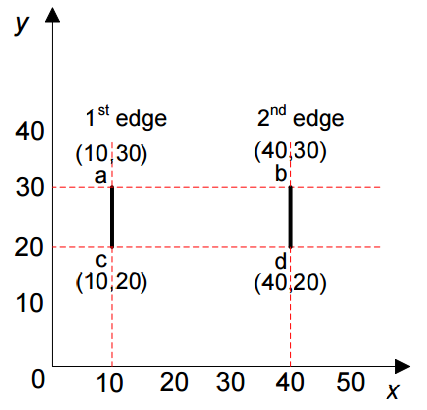
\includegraphics[scale=0.3]{edge_analysis_graphic.png}  
    \caption{Координаты боковых границ номера}
    \label{fig:domain:search:edges_analisys:edge_graphic}
\end{figure}

\begin{figure}[ht]
\centering
    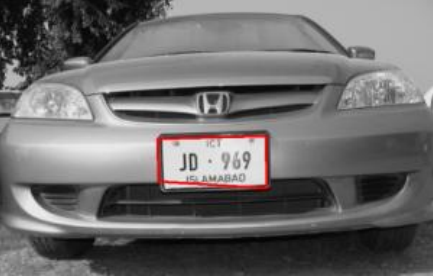
\includegraphics[scale=0.3]{edge_analysis_recognized_plate.png}  
    \caption{Распознанная граница номера}
    \label{fig:domain:search:edges_analisys:detected_edge}
\end{figure}

В своей работе автор не указывает на каком компьютере он запускал описанный выше алгоритм, но заявленное время работы при обработке изображений 640 х 480 пикселей 0,3 секунды, что делает его пригодным для работы в режиме реального времени. На тесте из 102 изображений, алгоритм нашел номера на 96 из них.

\subsection{Распознавание символов}
\label{sub:domain:imagerecognition}
Для распознавания отдельного символа лучше всего использовать перцептрон.
Перцептрон — математическая или компьютерная модель восприятия информации мозгом (кибернетическая модель мозга)~\cite{perceptron}.
Перцептрон состоит из трёх типов элементов, а именно: поступающие от сенсоров сигналы передаются ассоциативным элементам, а затем реагирующим элементам. Таким образом, перцептроны позволяют создать набор ассоциаций между входными стимулами и необходимой реакцией на выходе.

Элементарный перцептрон состоит из элементов 3-х типов: S-элементов, A-элементов и одного R-элемента. S-элементы — это слой сенсоров, или рецепторов. В физическом воплощении они соответствуют, например, светочувствительным клеткам сетчатки глаза или фоторезисторам матрицы камеры. Каждый рецептор может находиться в одном из двух состояний — покоя или возбуждения, и только в последнем случае он передаёт единичный сигнал в следующий слой, ассоциативным элементам.

A-элементы называются ассоциативными, потому что каждому такому элементу, как правило, соответствует целый набор (ассоциация) S-элементов. A-элемент активизируется, как только количество сигналов от S-элементов на его входе превысило некоторую величину $\theta$. Таким образом, если набор соответствующих S-элементов располагается на сенсорном поле в форме буквы "Д", A-элемент активизируется, если достаточное количество рецепторов сообщило о появлении «белого пятна света» в их окрестности, то есть A-элемент будет как бы ассоциирован с наличием/отсутствием буквы "Д" в некоторой области.

Сигналы от возбудившихся A-элементов, в свою очередь, передаются в сумматор R, причём сигнал от i-го ассоциативного элемента передаётся с коэффициентом $w_i$. Этот коэффициент называется весом A—R связи.

Так же как и A-элементы, R-элемент подсчитывает сумму значений входных сигналов, помноженных на веса. R-элемент, а вместе с ним и элементарный перцептрон, выдаёт 1, если линейная форма превышает порог $\theta$ иначе на выходе будет -1. Математически, функцию, реализуемую R-элементом, можно записать так:
$f(x) = sign(\sum_{i=1}^{n} w_i x_i - \theta)$
Обучение элементарного перцептрона состоит в изменении весовых коэффициентов $W_i$ связей A—R. Веса связей S—A (которые могут принимать значения $\{ -1, 0, 1 \}$) и значения порогов A-элементов выбираются случайным образом в самом начале и затем не изменяются.

После обучения перцептрон готов работать в режиме распознавания или обобщения. В этом режиме перцептрону предъявляются ранее неизвестные ему объекты, и перцептрон должен установить, к какому классу они принадлежат. Работа перцептрон состоит в следующем: при предъявлении объекта, возбудившиеся A-элементы передают сигнал R-элементу, равный сумме соответствующих коэффициентов $w_i$. Если эта сумма положительна, то принимается решение, что данный объект принадлежит к первому классу, а если она отрицательна — то ко второму.

\subsection{Примеры реализации}
\label{sub:domain:realization}

\subsubsection{}
\label{sub:domain:realization:automarshal}
Автомаршал – программное обеспечение для распознавания номеров автомобилей. Применяется для автоматизации парковок, весовых, КПП, автомоек, ТСЖ и т.п.\cite{auto_marshal}
Достоинства:
\begin{itemize}
  \item Имеются версии распознающие номера на скорости до 150 км/ч
  \item Поддерживаются номерные знаки большого количества стран: Российская Федерация, Казахстан, Украина, Белоруссия, Киргизия, Узбекистан, Нидерланды, Польша, Бельгия, Германия
\end{itemize}
Недостатки:
\begin{itemize}
  \item Интегрируется только с *.xls, *.xlsx, *.csv базами данных, т.е не подходит для компаний с развитой IT инфраструктурой
  \item Высокая цена, которая зависи от количества камер и стран, чьи регистрационные знаки распознаются
  \item Работает только на \windows{} серверах.
  \item Нет возможности попробовать перед покупкой.
\end{itemize}

\subsubsection{}
\label{sub:domain:}
Модуль распознавания автомобильных номеров - Альфа системз~\cite{alpha_system}. Модуль распознавания автомобильных номеров автоматически определяет и распознает номера автомобилей в поле зрения камеры. Он позволяет фиксировать и сохранять в базе данных SQL распознанный номер, а также изображение транспортного средства, часть кадра с номерным знаком и время регистрации. Таким образом, формируется база всех транспортных средств, прошедших через зону контроля, с возможностью добавления текстового комментария к каждому распознанному номеру. В совокупности с модулем «Радар», предоставляющем информацию о скорости автомобилей, модуль распознавания автомобильных номеров может использоваться ГИБДД для регистрации нарушителей скоростного режима. Есть возможность сравнения распознаваемых номеров со сторонней базой номеров (например, автомобилей, числящихся в угоне), что позволяет применять модуль для целей розыска. Другим важным применением модуля является его использование в системах автоматического учета и контроля доступа автотранспорта на охраняемые объекты и платные автостоянки.
Достоинства:
\begin{itemize}
  \item Работает с SQL базами данных
  \item Поддерживаются номерные знаки большого количества стран: Российской Федерации, Беларуси, Украины, Молдавии, Казахстана, Узбекистана, Латвии, Эстонии, Польши, Германии, Испании, Бразилии, Кубы.
\end{itemize}
Недостатки:
\begin{itemize}
  \item Возможность интеграции лучше чем у Автомаршала(\ref{sub:domain:realization:automarshal}) но все ещё не достаточно хороша: нет точки расширения для интегрирования с имеющимися rest сервисами компании.
  \item Высокая и непрозрачная цена.
  \item Работает только на \windows{} серверах.
  \item Нет возможности попробовать перед покупкой.
\end{itemize}

\subsubsection{}
Распознаватель авто номеров - autonomerok. Autonomerok - производит распознавание номера машины в потоке, сохранение события с записью номера, времени и кадра с номером, а также может управлять исполнительными устройствами. Программа будет отлично работать c аналоговыми IP видеокамерами разных производителей.
\begin{itemize}
  \item Работает с SQL light базой данных.
  \item Есть возможность проверить перед покупкой.
\end{itemize}
Недостатки:
\begin{itemize}
  \item Возможность интеграции лучше чем у Автомаршала(\ref{sub:domain:realization:automarshal}) но все ещё не достаточно хороша: нет точки расширения для интегрирования с имеющимися rest сервисами компании.
  \item Высокая цена.
  \item Работает только на \windows{} серверах.
  \item Небольшая количество по сравнению с Автомаршалом и Альфи системз, количество поддерживаемых типов номерных знаков.
\end{itemize}

\subsubsection{} Все имеющиеся приложения имеют высокую цену и лишний для нашей задачи функционал. Они позиционирую себя как готовые решения для платных парковок, авто моек и т.п. и расчитаны больше на малые компании и частных предпринимателей, у которых нет развитой IT инфраструктуры. 

\subsection{Постановка целей и задач дипломного проекта}
Цель - разработка программного средства для автоматизации автомобильной стоянки компании \company{}.


Задачи:
\begin{itemize}
  \item Разработка архитектуры ПС;
  \item Разработка алгоритмов;
  \item Выбор платформы для разработки программного средства;
  \item Разработка пользовательского интерфейса;
  \item Создание базового проекта в среде программирования;
  \item Создание пользовательского интерфейса;
  \item Программирование и тестирование модулей;
  \item Сборка и тестирование ПС;
\end{itemize}


%\lstset{style=fsharpstyle}

\section{Используемые технологии} 
\label{sec:practice:technology_used}

Выбор технологий является важным предварительным этапом разработки сложных информационных систем.
Платформа и язык программирования, на котором будет реализована система, заслуживает большого внимания, так как исследования показали, что выбор языка программирования влияет на производительность труда программистов и качество создаваемого ими кода~\cite[c.~59]{mcconnell_2005}.

Ниже перечислены некоторые факторы, повлиявшие на выбор технологий:
\begin{itemize}
\item Разрабатываемое ПО должно работать на операционной системе Windows~7 и более новых версиях системы.
\item Среди различных платформ разработки имеющийся программист лучше всего знаком с разработкой на платформе \dotnet{}.
\item Дальнейшей поддержкой проекта, возможно, будут заниматься разработчики, не принимавшие участие в выпуске первой версии.
\item Имеющийся разработчик имеет опыт работы с объекто"=ориентированными и с функциональными языками программирования.
\end{itemize}

Основываясь на опыте работы имеющихся программистов разрабатывать ПО целесообразно на платформе \dotnet{}.
Приняв во внимание необходимость обеспечения доступности дальнейшей поддержки ПО, возможно, другой командой программистов, целесообразно не использовать малоизвестные и сложные языки программирования.
С учетом этого фактора выбор языков программирования сужается до четырех официально поддерживаемых Microsoft и имеющих изначальную поддержку в Visual Studio~2012: \cppcli{}, \csharp{}, \vbnet{} и \fsharp{}.
Необходимость использования низкоуровневых возможностей \cppcli{} в разрабатываемом ПО отсутствует, следовательно данный язык можно исключить из списка кандидатов.
\vbnet{} уступает по удобству использования двум другим кандидатам из нашего списка.
Оставшиеся два языка программирования \csharp{} и \fsharp{} являются первостепенным, элегантными, мультипарадигменными языками программирования для платформы \dotnet.
Таким образом, с учетом вышеперечисленных факторов, целесообразно остановить выбор на следующих технологиях:
\begin{itemize}
  \item операционная система Windows~7;
  \item платформа разработки \dotnet{};
  \item языки программирования \csharp{} и \fsharp{}.
\end{itemize}
Для реализации поставленной задачи нет необходимости в использовании каких"=либо прикладных библиотек для создания настольных или веб"=приложений, достаточно использовать стандартные библиотеки указанных выше языков.
Поддержка платформой \dotnet{} различных языков программирования позволяет использовать язык, который наиболее просто и <<красиво>> позволяет решить возникающую задачу.
Разрабатываемое программное обеспечение в некоторой степени использует данное преимущество платформы.
Язык \csharp{} больше подходит для создания высокоуровнего дизайна проложения (иерархия классов и интерфейсов, организация пространств имен и публичного программного интерфейса), язык \fsharp{} "--- для реализации логики приложения, функций и методов~\cite{fsdg_2010}, прототипирования различных идей.
В разрабатываемом программном продукте \csharp{} используется для предоставления удобного программного интерфейса, \fsharp{} "--- для прототипирования и реализации вычислительной логики.
Далее проводится характеристика используемых технологий и языков программирования более подробно.



\subsection{Программная платформа \dotnet}
\label{sub:practice:microsoft_net}
Программная платформа \dotnet{} является одной из реализаций стандарта ECMA-335~\cite{ecma_335} и является современным инструментом создания клиентских и серверных приложений для операционной системы Windows.
Первая общедоступная версия \netfx{} вышла в феврале 2002 года.
С тех пор платформа активно эволюционировала и на данный момент было выпущено шесть версии данного продукта.
На данный момент номер последней версии \netfx{} "--- 4.5.
Платформа \dotnet{} была призвана решить некоторые наболевшие проблемы, скопившиеся на момент её выхода, в средствах разработки приложений под Windows. 
Ниже перечислены некоторые из них~\cite[с.~\Rmnum{14}\,--\,\Rmnum{17}]{richter_2007_ru}:
\begin{itemize}
  \item сложность создания надежных приложений;
  \item сложность развертывания и управления версиями приложений и библиотек;
  \item сложность создания переносимого ПО;
  \item отсутствие единой целевой платформы для создателей компиляторов;
  \item проблемы с безопасным исполнением непроверенного кода;
  \item великое множество различных технологий и языков программирования, которые не совместимы между собой.
\end{itemize}

Многие из этих проблем были решены.
Далее более подробно рассматривается внутреннее устройство \dotnet{}.

Основными составляющими компонентами \dotnet{} являются общая языковая исполняющая среда (Common Language Runtime) и стандартная библиотека классов (Framework Class Library).
CLR представляет из себя виртуальную машину и набор сервисов обслуживающих исполнение программ написанных для \dotnet{}.
Ниже приводится перечень задач, возлагаемых на CLR~\cite{marchenko_2007}:
\begin{itemize}
  \item загрузка и исполнение управляемого кода;
  \item управление памятью при размещении объектов;
  \item изоляция памяти приложений;
  \item проверка безопасности кода;
  \item преобразование промежуточного языка в машинный код;
  \item доступ к расширенной информации от типах "--- метаданным;
  \item обработка исключений, включая межъязыковые исключения;
  \item взаимодействие между управляемым и неуправляемым кодом (в том числе и COM"=объектами);
  \item поддержка сервисов для разработки (профилирование, отладка и т.\,д.).
\end{itemize}

Программы написанные для \dotnet{} представляют из себя набор типов взаимодействующих между собой.
\dotnet{} имеет общую систему типов (Common Type System, CTS).
Данная спецификация описывает определения и поведение типов создаваемых для \dotnet{}~\cite{richter_2012_en}.
В частности в данной спецификации описаны возможные члены типов, механизмы сокрытия реализации, правила наследования, типы"=значения и ссылочные типы, особенности параметрического полиморфизма и другие возможности предоставляемые CLI.
Общая языковая спецификация (Common Language Specification, CLS) "--- подмножество общей системы типов. 
Это набор конструкций и ограничений, которые являются руководством для создателей библиотек и компиляторов в среде \netfx{}.
Библиотеки, построенные в соответствии с CLS, могут быть использованы из любого языка программирования, поддерживающего CLS. 
Языки, соответствующие CLS (к их числу относятся языки \csharp{}, \vbnet{}, \cppcli{}), могут интегрироваться друг с другом. CLS "--- это основа межъязыкового взаимодействия в рамках платформы \dotnet{}~\cite{marchenko_2007}.

Некоторые из возможностей, предоставляемых \dotnet{}: верификация кода, расширенная информация о типах во время исполнения, сборка мусора, безопасность типов, "--- невозможны без наличия подробных метаданных о типах из которых состоит исполняемая программа.
Подробные метаданные о типах генерируются компиляторами и сохраняются в результирующих сборках.
Сборка "--- это логическая группировка одного или нескольких управляемых модулей или файлов ресурсов, является минимальной единицей с точки зрения повторного использования, безопасности и управлениями версиями~\cite[с.~6]{richter_2012_en}.

Одной из особенностей \dotnet{}, обеспечивающей переносимость программ без необходимости повторной компиляции, является представление исполняемого кода приложений на общем промежуточном языке (Common Intermediate Language, CIL). 
Промежуточный язык является бестиповым, стековым, объекто"=ориентированным ассемблером~\cite[с.~16\,--\,17]{richter_2012_en}.
Данный язык очень удобен в качестве целевого языка для создателей компиляторов и средств автоматической проверки кода для платформы \dotnet{}, также язык довольно удобен для чтения людьми.
Наличие промежуточного языка и необходимость создания производительных программ подразумевают наличие преобразования промежуточного кода в машинный код во время исполнения программы.
Одним из компонентов общей языковой исполняющей среды, выполняющим данное преобразование, является компилятор времени исполнения (Just-in-time compiler) транслирующий промежуточный язык в машинные инструкции, специфические для архитектуры компьютера на котором исполняется программа.

Ручное управление памятью всегда являлось очень кропотливой и подверженной ошибкам работой.
Ошибки в управлении памятью являются одними из наиболее сложных в устранении типами программных ошибок, также эти ошибки обычно приводят к непредсказуемому поведению программы, поэтому в \dotnet{} управление памятью происходит автоматически~\cite[с.~505\,--\,506]{richter_2012_en}.
Автоматическое управление памятью является механизмом поддержания иллюзии бесконечности памяти.
Когда объект данных перестает быть нужным, занятая под него память автоматически освобождается и используется для построения новых объектов данных.
Имеются различные методы реализации такого автоматического распределения памяти~\cite[с.~489]{sicp_2006_ru}.
В~\dotnet{} для автоматического управления памятью используется механизм сборки мусора (garbage collection).
Существуют различные алгоритмы сборки мусора со своими достоинствами и недостатками. 
В \dotnet{} используется алгоритм пометок (mark and sweep) в сочетании с различными оптимизациями, такими как, например, разбиение всех объектов по поколениям и использование различных куч для больших и малых объектов.

Ниже перечислены, без приведения подробностей, некоторые важные функции исполняемые общей языковой исполняющей средой:
\begin{itemize}
  \item обеспечение многопоточного исполнения программы;
  \item поддержание модели памяти, принятой в CLR;
  \item поддержка двоичной сериализации;
  \item управление вводом и выводом;
  \item структурная обработка исключений;
  \item возможность размещения исполняющей среды внутри других процессов.
\end{itemize}

Как уже упоминалось выше, большую ценностью для \dotnet{} представляет библиотека стандартных классов "--- соответствующая CLS"=спецификации объектно"=ориентированная библиотека классов, интерфейсов и системы типов (типов"=значений), которые включаются в состав платформы \dotnet{}.
Эта библиотека обеспечивает доступ к функциональным возможностям системы и предназначена служить основой при разработке .NET"=приложений, компонент, элементов управления~\cite{marchenko_2007}.



\subsection{Язык программирования \csharp{}}
\label{sub:practice:csharp_overview}
\csharp{} "--- объектно"=ориентированный, типо"=безопасный язык программирования общего назначения.
Язык создавался с целью повысить продуктивность программистов.
Для достижения этой цели в языке гармонично сочетаются простота, выразительность и производительность промежуточного кода, получаемого после компиляции.
Главным архитектором и идеологом языка с первой версии является Андрес Хейлсберг (создатель Turbo Pascal и архитектор Delphi).
Язык \csharp{} является платформенно нейтральным, но создавался для хорошей работы с \dotnet{}~\cite{albahari_2012_en}.
Этот язык сочетает простой синтаксис, похожий на синтаксис языков \cpp{} и \java{}, и полную поддержку всех современных объектно-ориентированных концепций и подходов. В качестве ориентира при разработке языка было выбрано безопасное программирование, нацеленное на создание надежного и простого в сопровождении кода~\cite{volosevich_cs_2011}.

Язык имеет богатую поддержку парадигмы объекто"=ориентированного программирования, включающую поддержку инкапсуляции, наследования и полиморфизма.
Отличительными чертами \csharp{} с точки зрения ОО парадигмы являются:
\begin{itemize}
  \item Унифицированная система типов. 
        В \csharp{} сущность, содержащая данные и методы их обработки, называется типом.
        В \csharp{} все типы, являются ли они пользовательскими типами, или примитивами, такими как число, производны от одного базового класса.
  \item Классы и интерфейсы.
        В классической объекто"=ориентированной парадигме существуют только классы.
        В \csharp{} дополнительно существуют и другие типы, например, интерфейсы.
        Интерфейс "--- это сущность напоминающая классы, но содержащая только определения членов.
        Конкретная реализация указанных членов интерфейса происходит в типах, реализующих данный интерфейс.
        В частности интерфейсы могут быть использованы при необходимости проведения множественного наследования (в отличие от языков \cpp{} и Eiffel, \csharp{} не поддерживает множественное наследование классов).
  \item Свойства, методы и события.
        В чистой объекто"=ориентированной парадигме все функции являются методами.
        В \csharp{} методы являются лишь одной из возможных разновидностей членов типа, в \csharp{} типы также могут содержать свойства, события и другие члены.
        Свойство "--- это такая разновидность функций, которая инкапсулирует часть состояния объекта.
        Событие "--- это разновидность функций, которые реагируют на изменение состояния объекта~\cite{albahari_2012_en}.
\end{itemize}

В большинстве случаев \csharp{} обеспечивает безопасность типов в том смысле, что компилятор контролирует чтобы взаимодействие с экземпляром типа происходило согласно контракту, который он определяют.
Например, компилятор \csharp{} не скомпилирует код который обращается со строками, как если бы они были целыми числами.
Говоря более точно, \csharp{} поддерживает статическую типизацию, в том смысле что большинство ошибок типов обнаруживаются на стадии компиляции.
За соблюдение более строгих правил безопасности типов следит исполняющая среда.
Статическая типизация позволяет избавиться от широкого круга ошибок, возникающих из-за ошибок типов. 
Она делает написание и изменение программ более предсказуемыми и надежными, кроме того, статическая типизация позволяет существовать таким средствам как автоматическое дополнение кода и его предсказуемый статический анализ.
Еще одним аспектом типизации в \csharp{} является её строгость.
Строгая типизация означает, что правила типизации в языке очень <<сильные>>.
Например, язык не позволяет совершать вызов метода, принимающего целые числа, передавая в него вещественное число~\cite{albahari_2012_en}. 
Такие требования спасают от некоторых ошибок.

\csharp{} полагается на автоматическое управление памятью со стороны исполняющей среды, предоставляя совсем немного средств для управления жизненным циклом объектов.
Не смотря на это, в языке все же присутствует поддержка работы с указателями.
Данная возможность предусмотрена для случаев, когда критически важна производительность приложения или необходимо обеспечить взаимодействие с неуправляемым кодом~\cite{albahari_2012_en}. 

Как уже упоминалось \csharp{} не является платформенно зависимым языком.
Благодаря усилиям компании Xamarin возможно писать программы на языке \csharp{} не только для операционных систем Microsoft, но и ряда других ОС.
Существуют инструменты создания приложений на \csharp{} для серверных и мобильных платформ, например: iOS, Android, Linux и других.

Создатели языка \csharp{} не являются противниками привнесения в язык новых идей и возможностей, в отличии от создателей одного из конкурирующих языков.
Каждая новая версия компилятора языка привносит различные полезные возможности, которые отчаются требованиям индустрии. 
Далее приводится краткий обзор развития языка.

Первая версия \csharp{} была похожа по своим возможностям на \java{} 1.4, несколько их расширяя: так, в \csharp{} имелись свойства (выглядящие в коде как поля объекта, но на деле вызывающие при обращении к ним методы класса), индексаторы (подобные свойствам, но принимающие параметр как индекс массива), события, делегаты, циклы \lstinline!foreach!, структуры, передаваемые по значению, автоматическое преобразование встроенных типов в объекты при необходимости (boxing), атрибуты, встроенные средства взаимодействия с неуправляемым кодом (DLL, COM) и прочее~\cite{csharp_wiki_2013_ru}. 

Версия \dotnet{} 2.0 привнесла много новых возможностей в сравнении с предыдущей версией, что отразилось и на языках под эту платформу.
Проект спецификации \csharp{} 2.0 впервые был опубликован Microsoft в октябре 2003 года; в 2004 году выходили бета"=версии (проект с кодовым названием Whidbey), \csharp{} 2.0 окончательно вышел 7 ноября 2005 года вместе с Visual Studio 2005 и \dotnet{} 2.0. 
Ниже перечислены новые возможности в версии 2.0
\begin{itemize}
  \item Частичные типы (разделение реализации класса более чем на один файл).

  \item Обобщённые, или параметризованные типы (generics). 
  В отличие от шаблонов \cpp{}, они поддерживают некоторые дополнительные возможности и работают на уровне виртуальной машины.
  Вместе с тем, параметрами обобщённого типа не могут быть выражения, они не могут быть полностью или частично специализированы, не поддерживают шаблонных параметров по умолчанию, от шаблонного параметра нельзя наследоваться.

  \item Новая форма итератора, позволяющая создавать сопрограммы с помощью ключевого слова \lstinline[style=csharpinlinestyle]!yield!, подобно Python и Ruby.
  
  \item Анонимные методы, обеспечивающие функциональность замыканий.

  \item Оператор ??: \lstinline!return obj1 ?? obj2;! означает (в нотации \csharp{} 1.0) \lstinline[style=csharpinlinestyle]/return obj1!=null ? obj1 : obj2;/.

  \item Обнуляемые (nullable) типы"=значения (обозначаемые вопросительным знаком, например, \lstinline[style=csharpinlinestyle]!int? i = null;!), представляющие собой те же самые типы-значения, способные принимать также значение null. 
  Такие типы позволяют улучшить взаимодействие с базами данных через язык SQL.

  \item Поддержка 64-разрядных вычислений позволяет увеличить адресное пространство и использовать 64-разрядные примитивные типы данных~\cite{csharp_wiki_2013_ru}.
\end{itemize}

Третья версия языка имела одно большое нововведение "--- Language Integrated Query (LINQ), для реализации которого в языке дополнительно появилось множество дополнительных возможностей. 
Ниже приведены некоторые из них:
\begin{itemize}
  \item Ключевые слова \lstinline[style=csharpinlinestyle]!select!, \lstinline[style=csharpinlinestyle]!from!, \lstinline[style=csharpinlinestyle]!where!, позволяющие делать запросы из SQL, XML, коллекций и т.\,п.

  \item Инициализацию объекта вместе с его свойствами:
  \begin{lstlisting}[style=csharpinlinestyle]
Customer c = new Customer(); c.Name = "James"; c.Age=30;
  \end{lstlisting}
  можно записать как
  \begin{lstlisting}[style=csharpinlinestyle]
Customer c = new Customer { Name = "James", Age = 30 };
  \end{lstlisting}

  \item Лямбда-выражения:
  \begin{lstlisting}[style=csharpinlinestyle]
listOfFoo.Where(delegate(Foo x) { return x.size > 10; });
  \end{lstlisting}
  теперь можно записать как
  \begin{lstlisting}[style=csharpinlinestyle]
listOfFoo.Where(x => x.size > 10);
  \end{lstlisting}

  \item Деревья выражений "--- лямбда-выражения теперь могут быть представлены в виде структуры данных, доступной для обхода во время выполнения, тем самым позволяя транслировать строго типизированные \csharp{}-выражения в другие домены (например, выражения SQL).

  \item Вывод типов локальной переменной: \lstinline[style=csharpinlinestyle]!var x = "hello";! вместо \lstinline[style=csharpinlinestyle]!string x = "hello";!

  \item Безымянные типы: \lstinline[style=csharpinlinestyle]!var x = new { Name = "James" };!

  \item Методы-расширения "--- добавление метода в существующий класс с помощью ключевого слова \lstinline[style=csharpinlinestyle]!this! при первом параметре статической функции.

  \item Автоматические свойства: компилятор сгенерирует закрытое  поле и соответствующие аксессор и мутатор для кода вида
  \begin{lstlisting}[style=csharpinlinestyle]
public string Name { get; private set; }
  \end{lstlisting}

\end{itemize}
\csharp{} 3.0 совместим с \csharp{} 2.0 по генерируемому MSIL-коду; улучшения в языке "--- чисто синтаксические и реализуются на этапе компиляции~\cite{csharp_wiki_2013_ru}.

\vbnet{} 10.0 и \csharp{} 4.0 были выпущены в апреле 2010 года, одновременно с выпуском Visual Studio 2010.
Новые возможности в версии 4.0:
\begin{itemize}
  \item Возможность использования позднего связывания.
  \item Именованные и опциональные параметры.
  \item Новые возможности COM interop.
  \item Ковариантность и контрвариантность интерфейсов и делегатов.
  \item Контракты в коде (Code Contracts)~\cite{csharp_wiki_2013_ru}.
\end{itemize}

В \csharp{} 5.0 было немного нововведений, но они носят большую практическую ценность.
В новой версии появилась упрощенная поддержка выполнения асинхронных функций с помощью двух новых слов "---  \lstinline[style=csharpinlinestyle]!async! и \lstinline[style=csharpinlinestyle]!await!.
Ключевым словом \lstinline[style=csharpinlinestyle]!async! помечаются методы и лямбда"=выражения, которые внутри содержат ожидание выполнения асинхронных операций с помощью оператора \lstinline[style=csharpinlinestyle]!await!, который отвечает за преобразования кода метода во время компиляции.


%\include{sec_arch_and_mod}

%\include{sec_ot}

%\include{sec_econ}

%\sectioncentered*{Заключение}
\addcontentsline{toc}{section}{Заключение}

В данном дипломном проекте был рассмотрен вопрос автоматизации распознавания номерных знаков автомобиля для корпоративной стоянки. В рамках проекта была рассмотрена теория по вопросу распознавания, разработанны алгоритмы архитектура програмного средства. Был реализован расширяемый программный продукт предназначенный для интеграции в развитую информационную инфраструктуру представляющий из себя клиент-серверное веб приложение. Была произведенна сборка и тестирование.



%% Зачем: Изменение надписи для списка литературы
% Почему: Пункт 2.8.1 Требований по оформлению пояснительной записки.
\renewcommand{\bibsection}{\sectioncentered*{Cписок использованных источников}}
\phantomsection\pagebreak% исправляет нумерацию в документе и исправляет гиперссылки в pdf
\addcontentsline{toc}{section}{Cписок использованных источников}

% Зачем: Печать списка литературы. База данных литературы - файл bibliography_database.bib
\bibliography{bibliography_database}


% \includepdf позволяет включить в результирующий pdf документ часть другого pdf документа, сделанного
% например не с помощью TeX. Бывает полезно, если какие-то диаграммны нарисованы, например, с помощью 
% Microoft Office и сохранены в pdf.
%\includepdf[pages={-}]{documents_list.pdf}

\end{document}
